\documentclass[20 pts]{article}
\usepackage{xeCJK}
\usepackage{amsfonts}
\usepackage{amssymb}
\usepackage{amsmath}
\usepackage{bm}
\setCJKmainfont{SimSun}
\title{ターボ符号器における決定論的インタリーバの設計に関する研究} 
\author{Kwame Ackah Bohulu}
\date{2017/10/12}
\begin{document}
\maketitle

\newpage
\begin{center}
\begin{figure}
		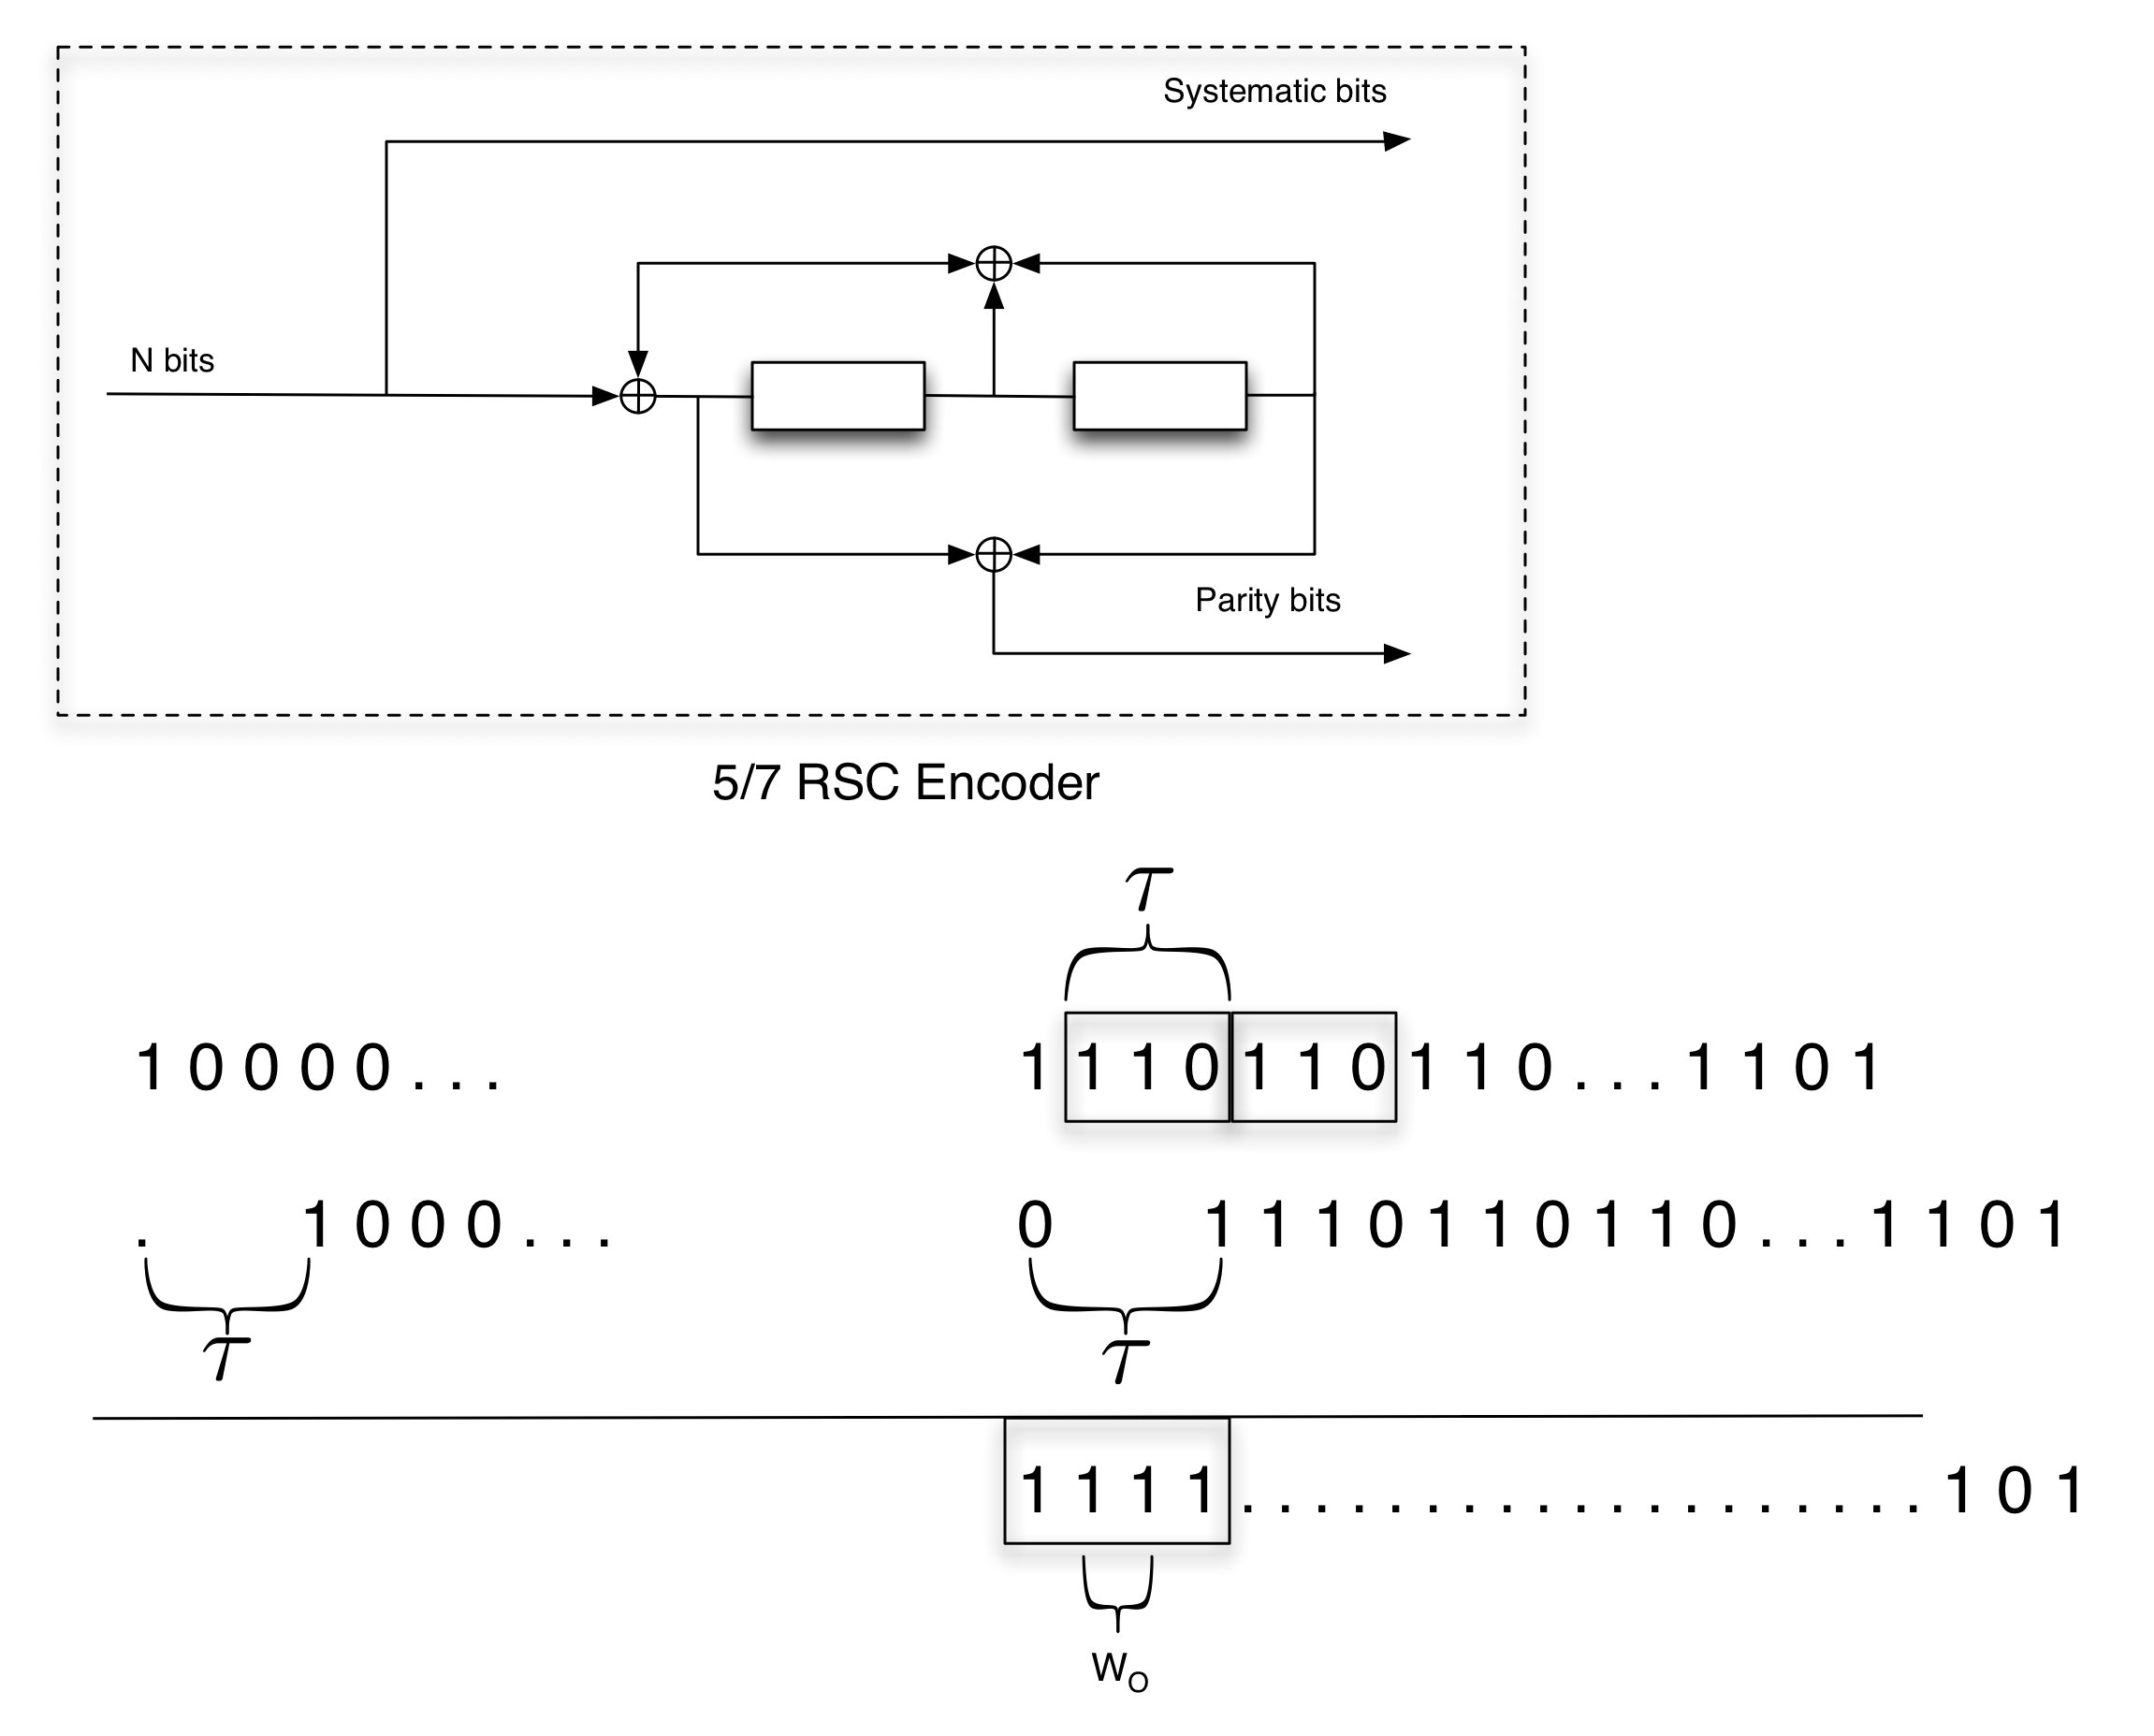
\includegraphics[width=\textwidth]{RSCExample2.jpg}
		\caption{5/7 RSC 符号器}
		\end{figure}
	\end{center}

\begin{center}
\begin{figure}
		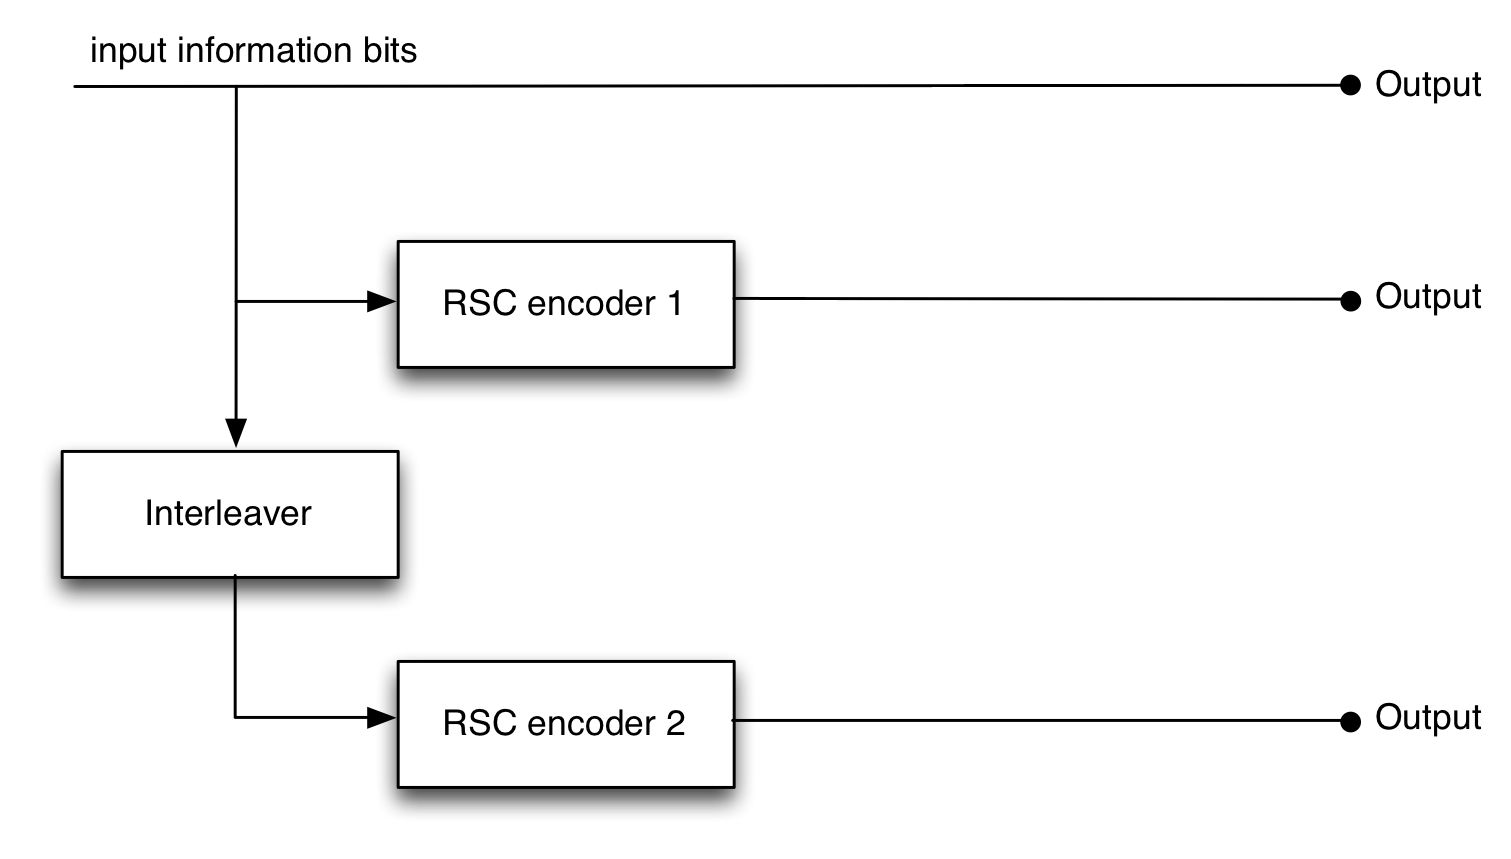
\includegraphics[width=\textwidth]{TurboEncoderNew.jpg}
		\caption{ターボ符号器}
		\end{figure}
	\end{center}
	
	
	\begin{center}
	\begin{figure}
		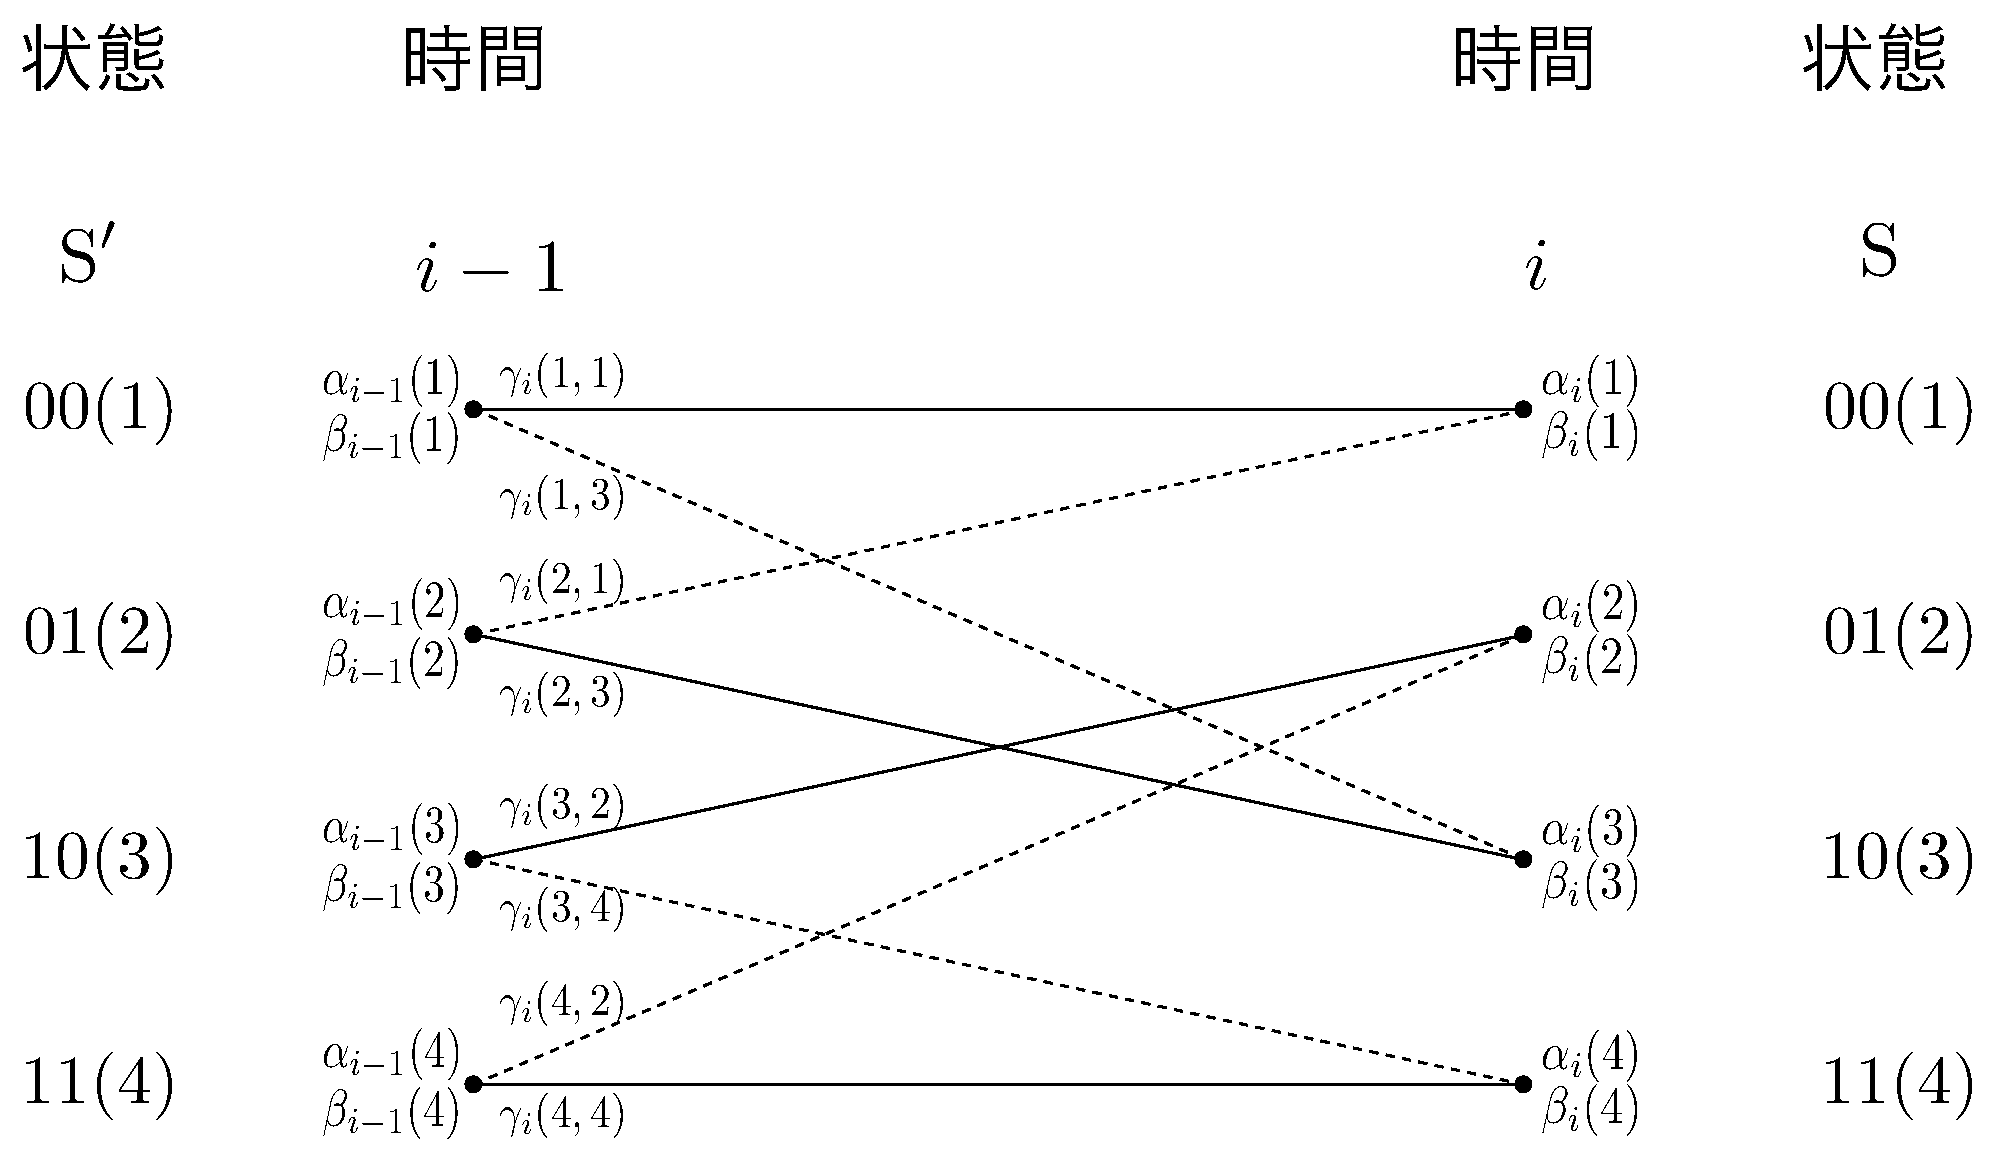
\includegraphics[width=\textwidth]{figure3.pdf}
		\caption{5/7 RSC 符号のTrellis図}
		\end{figure}
	\end{center}
	
	\begin{center}
	\begin{figure}
		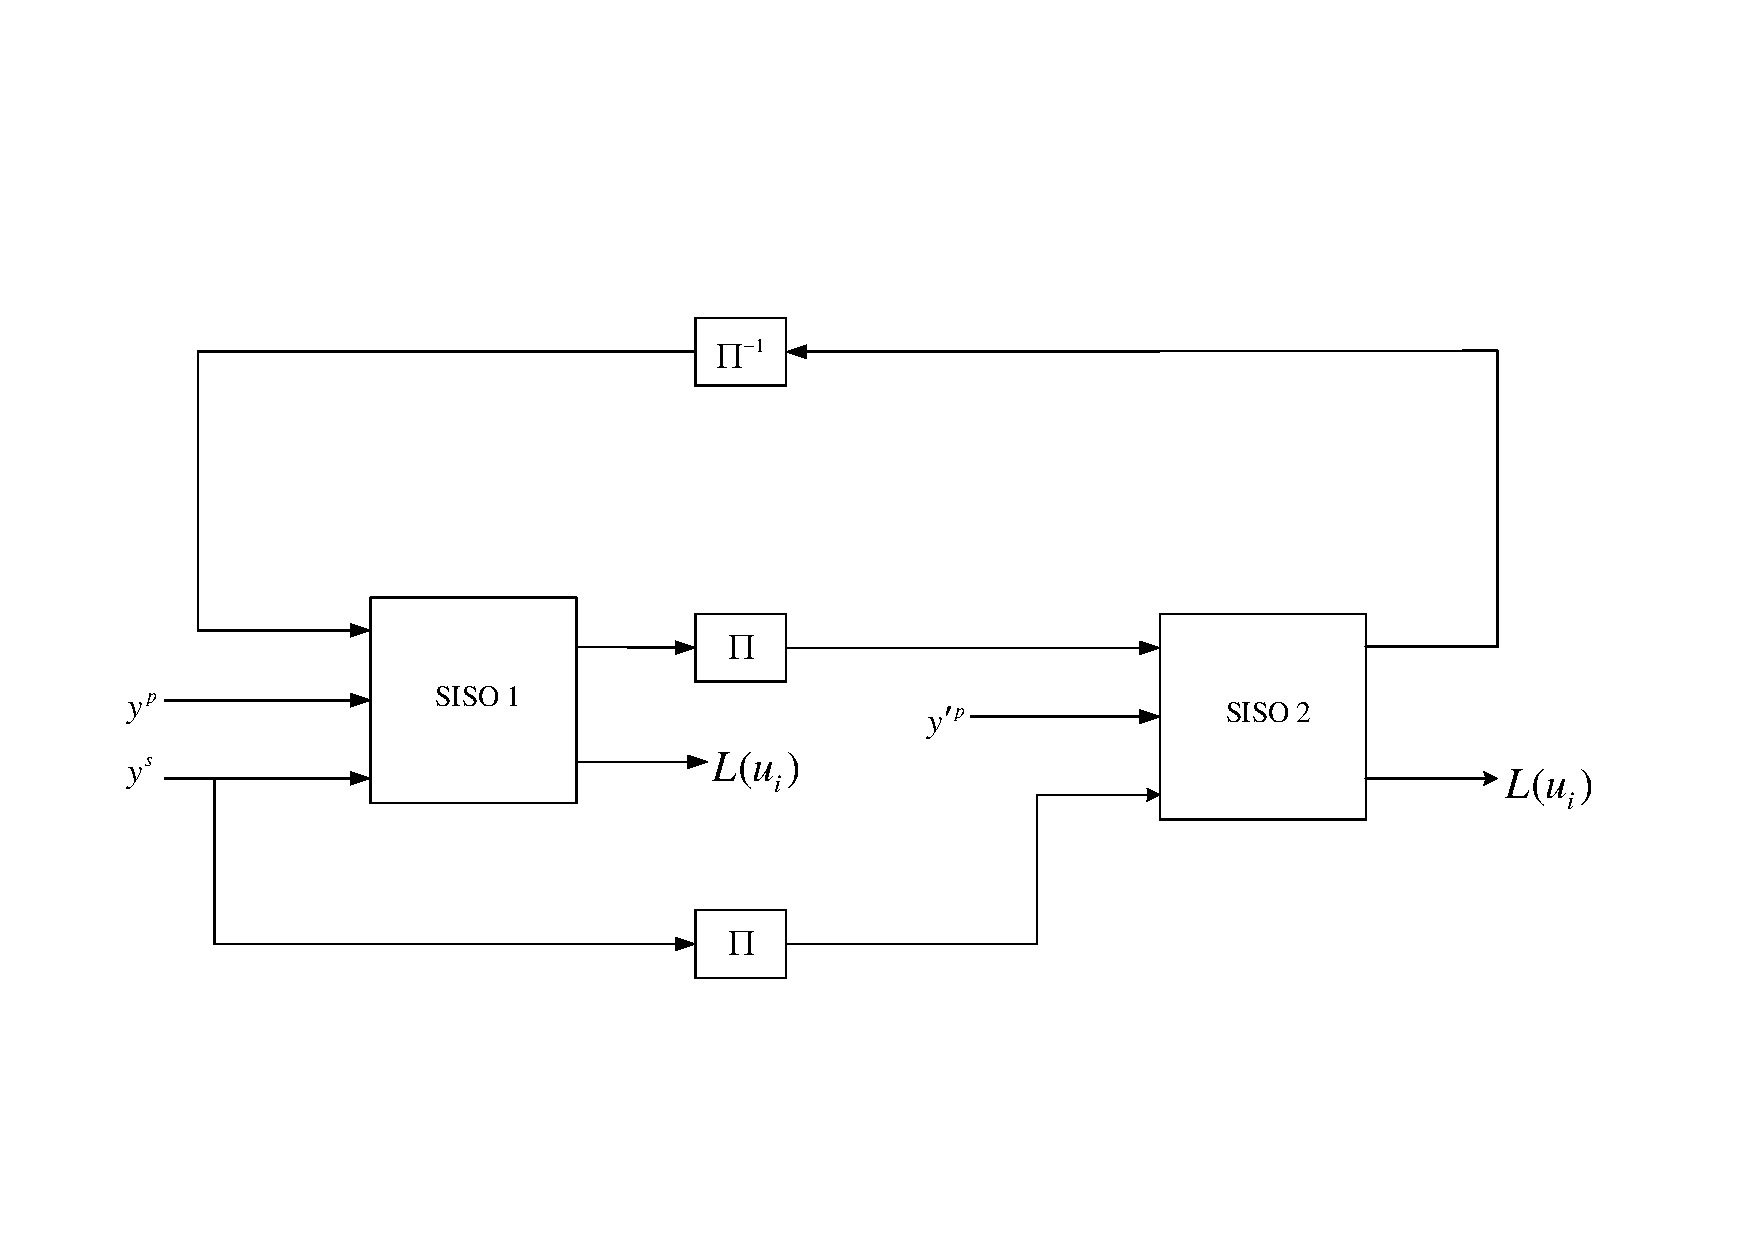
\includegraphics[width=\textwidth]{D1.pdf}
		\caption{ターボ復号器}
		\end{figure}
	\end{center}
\end{document}